\documentclass[11pt,a4paper]{article}
\usepackage[paper=a4paper,width=15cm,left=30mm,height=22cm]{geometry}

\usepackage{xltxtra}
\setmainfont[Mapping=tex-text]{Bitter}
\usepackage{setspace}
\linespread{1.20}
\setlength{\parskip}{0.5em}
\setlength{\parindent}{0em}

\usepackage[german]{babel}
\usepackage{graphicx}
\usepackage{acronym}

\usepackage{hyperref}
\usepackage[usenames,dvipsnames]{xcolor}
\hypersetup{
    bookmarks=true, % Test
    colorlinks=true,
    linkcolor=NavyBlue,
    citecolor=NavyBlue,
    urlcolor=NavyBlue
}

\begin{document}
\author{Markus Tacker}
\title{Bachelor-Thesis - Aufbau und Zeitplan}

\begin{center}

\begin{huge}Bachelor-Thesis\end{huge}

\bigskip

Aufbau und Zeitplan

\begin{small}Markus Tacker\\
\today

\end{small}

\end{center}

\section{Aufbau}

\begin{enumerate}
\item Abstract
\item Problem-Analyse
\begin{enumerate}
\item Definition -- was sind „Texte in Medienprodukten“
\item Texte in Medienprodukten -- Besonderheiten, Beteiligte, Workflow
\item Microsoft Office als Standard -- Analyse der Vorteile, verwendete Funktionen
\item Beispiele aus der Praxis
\item Schlussfolgerung
\end{enumerate}
\item Konzeption eines an die spezifischen Probleme angepassten Workflows
\begin{enumerate}
\item Vorraussetzung / Abgrenzung
\item Workflow -- Beschreibung des optimalen Workflows und die Rolle der Beteiligten
\item Beschreibung der notwendigen Funktionalität -- Unterteilung in Muss- und Kann-Kriterien
\item Nachteile/Risiken des Konzepts
\item Personas -- Vorstellung (basierend auf Interviews mit realen Personen), Analyse des Konzepts in Bezug auf Personas
\end{enumerate}

\item Entwurf einer Anwendung
\begin{enumerate}
\item Schnittstellen -- Anforderungen, Umfang, Ausprägung für Import-, Export- und Benachrichtigungsschnittstellen
\item Grundüberlegung zu einer GUI -- Anforderungen, Grundsätze, Usability, Aufbau, Wireframes
\end{enumerate}

\item Implementierung des Konzepts
\begin{enumerate}
\item Abgrenzung
\item Beschreibung der gewählten Umsetzung, Komponenten
\item Anwendung der Umsetzung am Beispiel des Studiengangsflyers
\end{enumerate}

\item Fazit
\end{enumerate}

\section{Personas}

Dies sind die Kollegen, die ich zur Erstellung der Personas und zu Hintergrund-Infos für das Konzept interviewen möchte (vorbehaltlich deren Zusage).

\begin{table}[htb]
\begin{tabular}{l l}

\textit{Name} & \textit{Titel} \\
\textit{Expertise} & \textit{Firma} \\

\hline

Sebastian Nell & Director of USE // Connected Products  \\
Projektleiter & Scholz \& Volkmer GmbH \\

\hline

Carsten Fischer & UX Designer \& Informationsarchitekt   \\
Informationsarchitekt & triplesense GmbH \\

\hline

Eva Kümml & Senior Konzept / User Experience \\
Konzept & SinnerSchrader Deutschland GmbH \\

\hline

Matthias Muck & Senior Digital Media Producer  \\
Reinzeichnung & BlueMars GmbH  \\

\hline

Sebastian Beyer & Developer  \\
Softwareentwicklung & Scholz \& Volkmer GmbH \\

\hline

Tobias Rudolphi & Lead Software Architect  \\
Integration & Zühlke Engineering GmbH \\

\end{tabular}
\caption{Interview-Partner Personas}
\end{table}

zusätzlich mindestens je eine weitere Person für Projektleitung auf Kundenseite und Texterstellung/Übersetzung.

\section{Zeitplan}

\begin{table}[htb]
\begin{tabular}{l l l}
Beginn & Montag, 26. März 2012 & \\
\hline
Problem-Analyse und Konzept & Montag, 26. März 2012 & bis Dienstag, 8. Mai 2012 \\
Implementierung & Mittwoch, 9. Mai 2012 & bis Freitag, 1. Juni 2012 \\
Version 1.0 & Mittwoch, 6. Juni 2012 & \\
Druck & Donnerstag, 21. Juni 2012 & \\
\hline
Abgabe & Montag, 25. Juni 2012 & \\
\end{tabular}
\caption{Zeitplan}
\end{table}

\begin{figure}[htb]
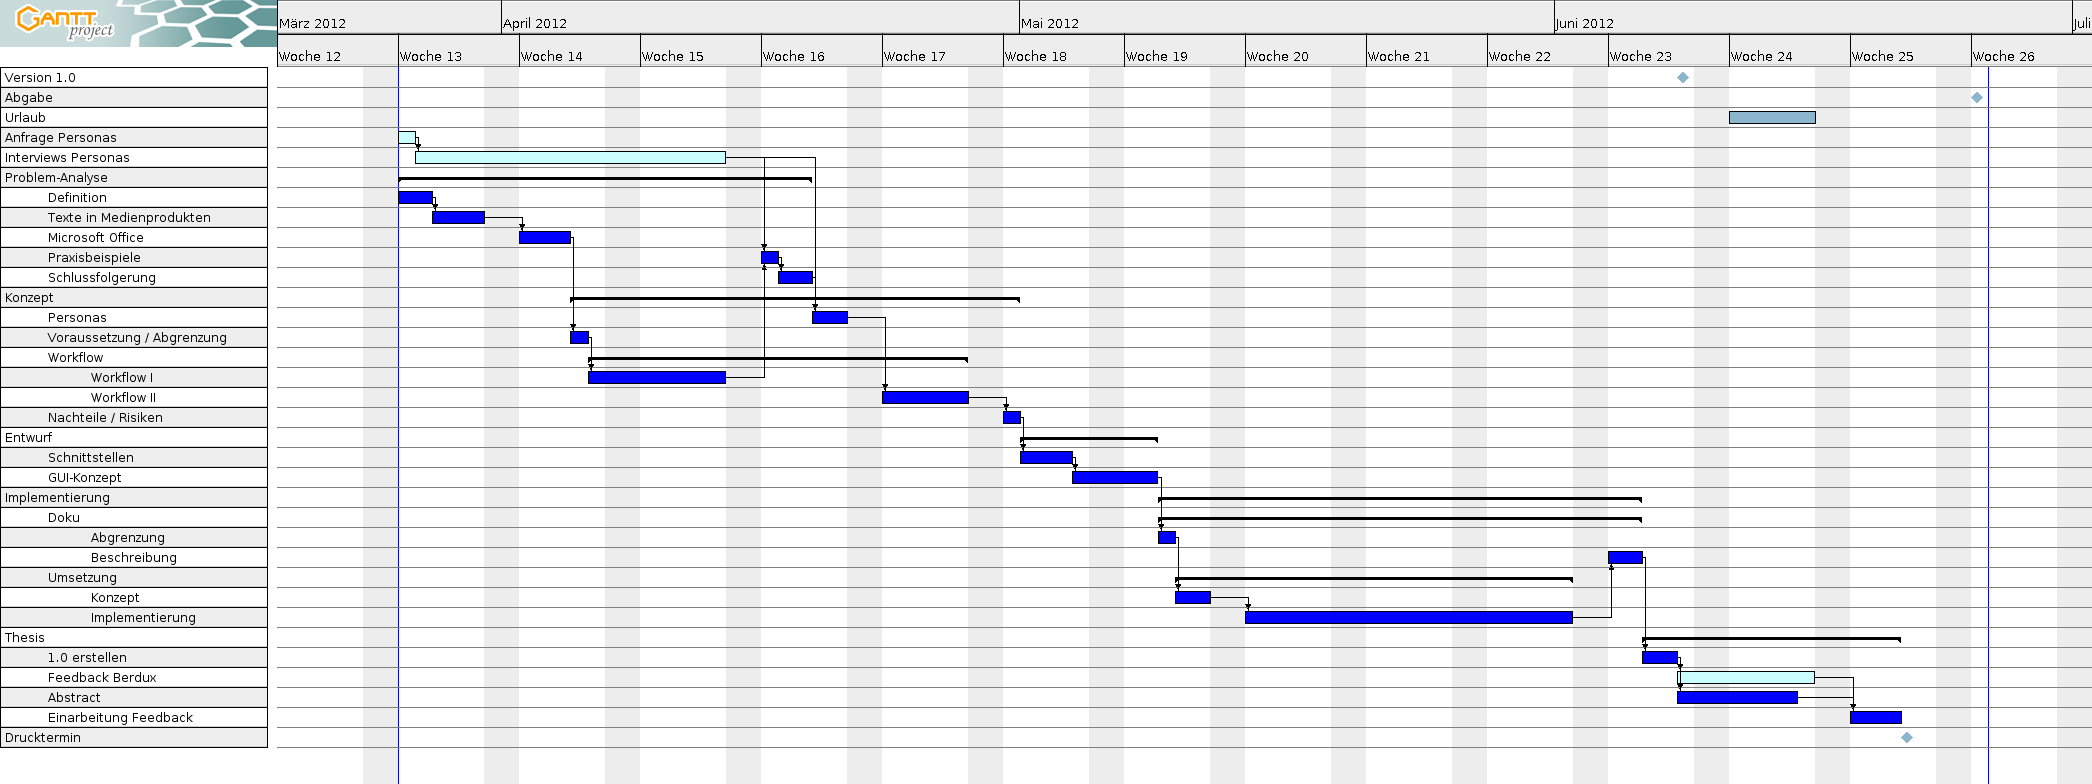
\includegraphics[width=\textwidth]{zeitplan.png}
\caption{Zeitplan als Gantt-Diagramm}
\end{figure}

\end{document}
